\chapter{Implementação}



\section{Web scraper}

Após uma reunião com o cliente foi percebido que o catálogo de produtos Motorline não se encontra em um
servidor, esta informação encontra-se apenas diretamente no website da empresa, sendo assim viu-se a 
necessidade de criar um web scraper.

Web scraping é uma terminologia dada para o processo de obter uma página web, ler a página e obter
dados desta, geralmente utilizando bots. O grande problema com web scraping é que pode ser facilmente
detetado. Tendo em conta este problema surgiram duas grandes formas principais de realizar web scraping,
a mais comum sendo realizar um pedido para obter uma página web e ler então esta, sendo assim um processo
rápido e simples. A segunda forma de realizar web scraping é através da simulação da ação humana 
conseguindo abrir o navegador pesquisar pela página desejada, descarregar a página e daí ler esta, 
tornando-se então em um processo lento e complexo.A grande diferença entre estas duas formas é a 
velocidade, visto que a segunda forma tem de esperar que o navegador inicie, de seguida terá de 
esperar que a página carregue e apenas após este processo poderá ser lida a página web.

Na reunião mencionada anteriormente foi decidido que o web scraper iria apenas correr 1 vez por mês
de forma a evitar a sobrelotação do servidor, não existindo problema visto que o catálogo não é 
atualizado regularmente. Para agilizar a realização do web scraper foi disponibilidado pela 
empresa a estrutura do website a seguir para obter as informações da página web.

\newpage

\subsection{Implemenção web scraper}
De forma a implementar e testar o web scraper sem sobrelotar o servidor, foi então descarregado todo
o wesite localmente, conseguindo assim simular o mesmo.

Para implementar o web scraper foi optado pela abordagem mais simples, realizar um pedido para obter a
pagina web, ler a página para obter os dados e guardar os dados.

Para isto foi optado pela linguagem python devido à facilidade desta lidar com grandes quantidades 
de dados. De forma a facilitar a localização dos dados na página foi utilizada a biblioteca bs4, também
conhecida como beautiful soup, esta biblioteca permite alimentar com uma página web e de seguida realizar
pesquisas sobre esta página baseado em tags e atributos dos elementos.

Tendo esta base em conta foi então primeiramente estudado que dados seriam necessários, sendo estes então:
\begin{enumerate}
    \item Categorias e subcategorias de produtos;
    \item Produtos de cada categoria e subcategoria;
    \item Documentação dos produtos;
    \item Imagens e videos dos produtos;
\end{enumerate}

\newpage

Para guardar estes dados foi utilizado um dicionário que contém primeiramente como chaves as categorias de produtos,
para cada categoria contém mais um dicionário com as subcategorias de produtos e para cada categoria existe uma lista
de produtos, contendo o nome de produto, imagem de amostra e url do mesmo.Por fim a chave produtos contém a lista de 
todos os produtos, sendo cada produto representado também por um dicionário, que contém como chaves os atributos do mesmo.
A utilização dicionarios e listas para guardar estes dados deve-se a que o objetivo será guardar estes dados 
em json e a transformação é simplificada utilizando estas estruturas devido à sua proximidade com a estrutura
json.

\begin{figure}[htb]
    \centering
    
    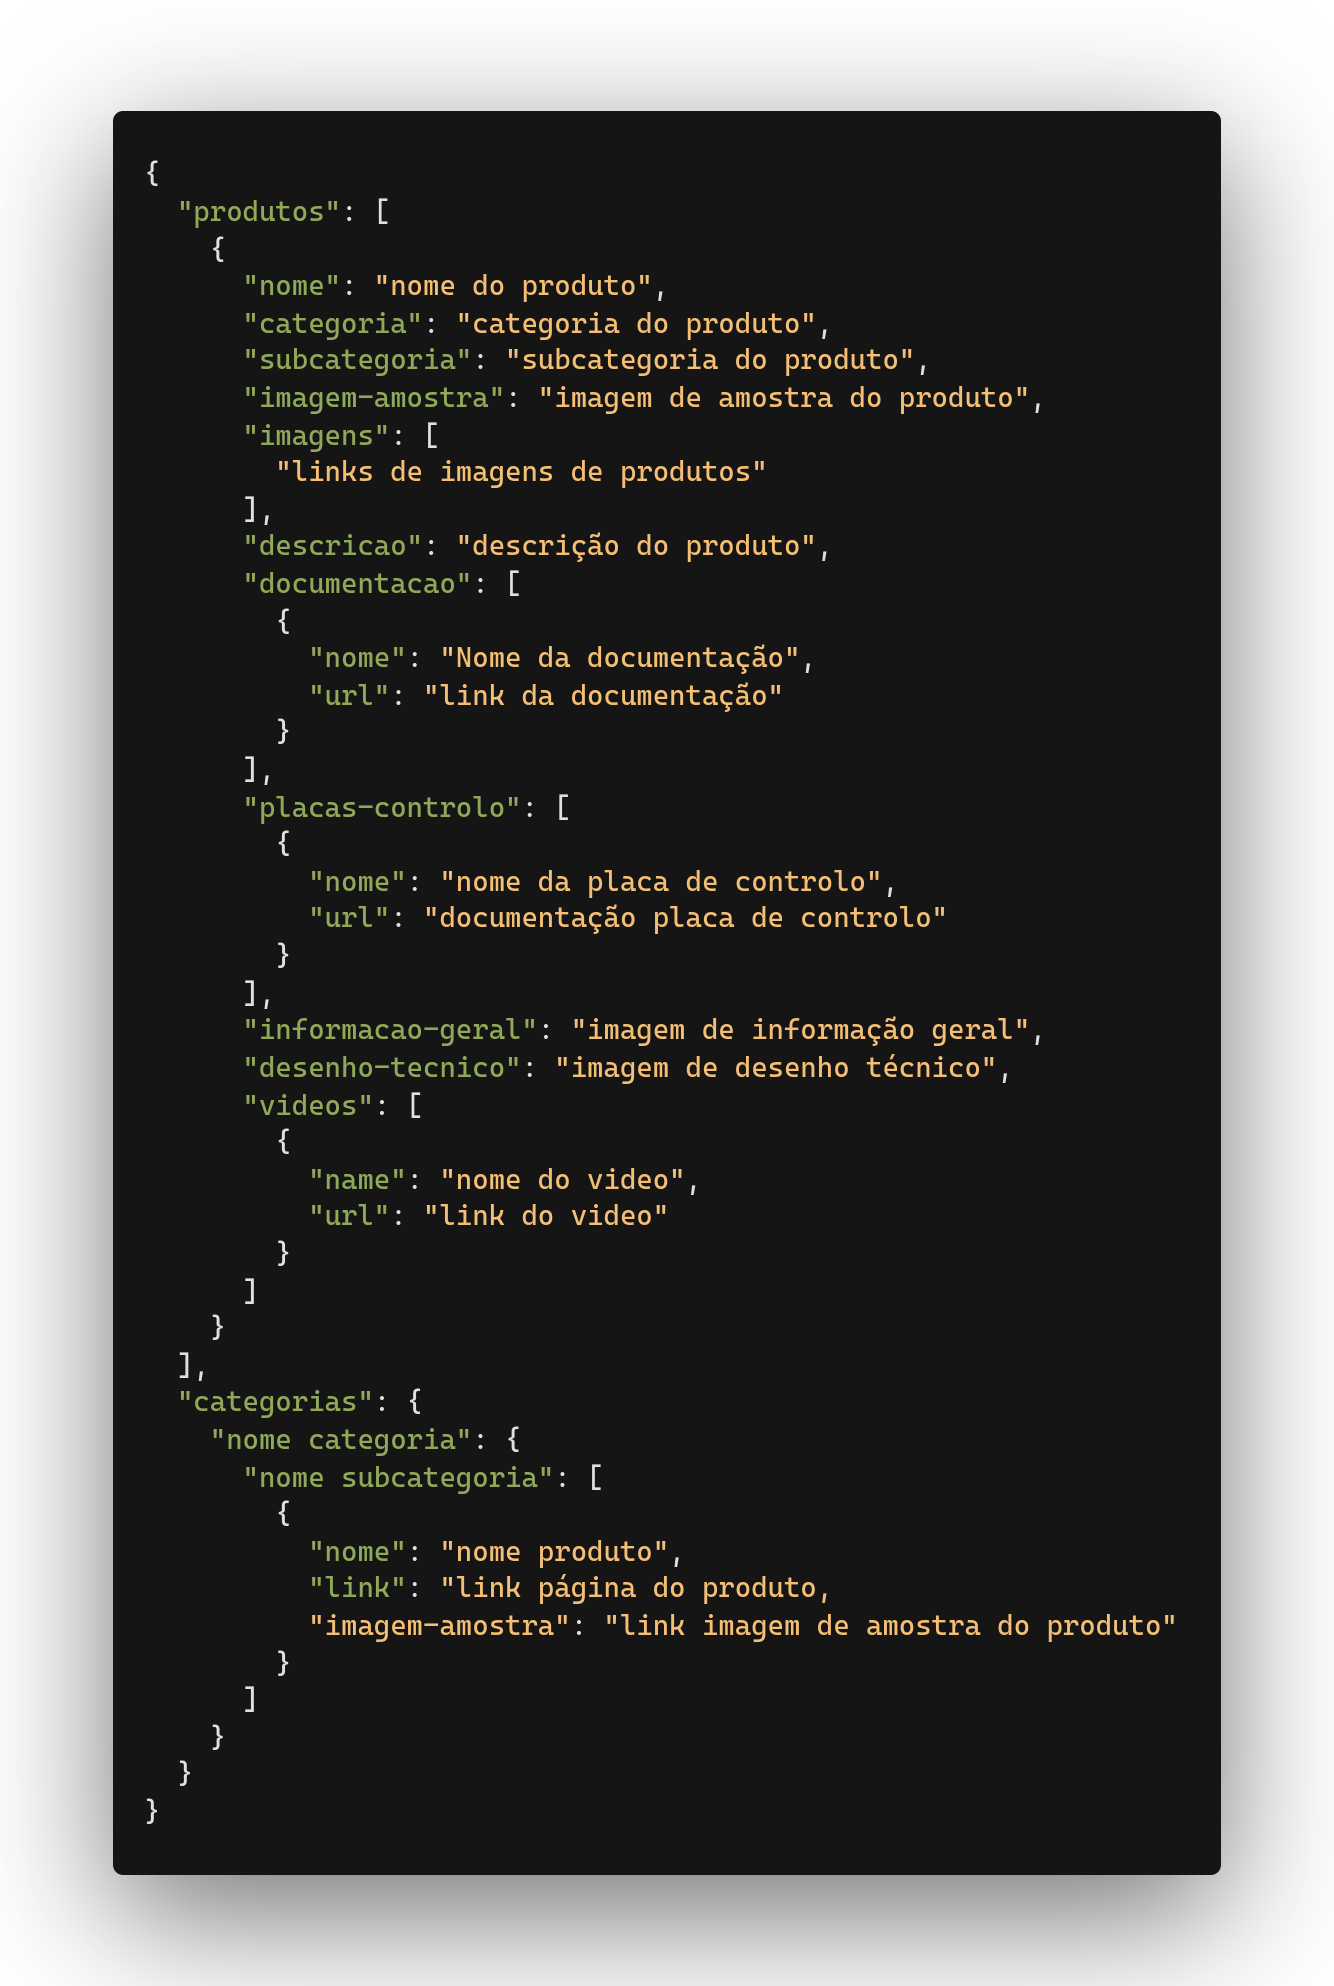
\includegraphics[width=0.7\textwidth]{images/implementacao/scraper/estrutura_scraper.png}
    \caption{Estrutura dos dados obtidos}
    \label{fig:49}
\end{figure}

\newpage

Após uma análise da estrutura do website foi percebido que a página geral de produtos possui todas as categorias
de produtos, assim como também as subcategorias de produtos com urls para as páginas que contém todos os produtos
das subcategorias. Sendo assim foi primeiramente percebido que cada conjunto é uma secção, pelo que é obtido
todas as secções de categorias e para cada uma destas secções é obtido o título da secção que equivale ao nome da
categoria e também todos os correspondentes a clicáveis. Os clicáveis corresponde às subcategorias de cada categoria
estes clicáveis contém também um url que redireciona para a página de produtos da subcategoria.

\begin{figure}[htb]
    \centering
    
    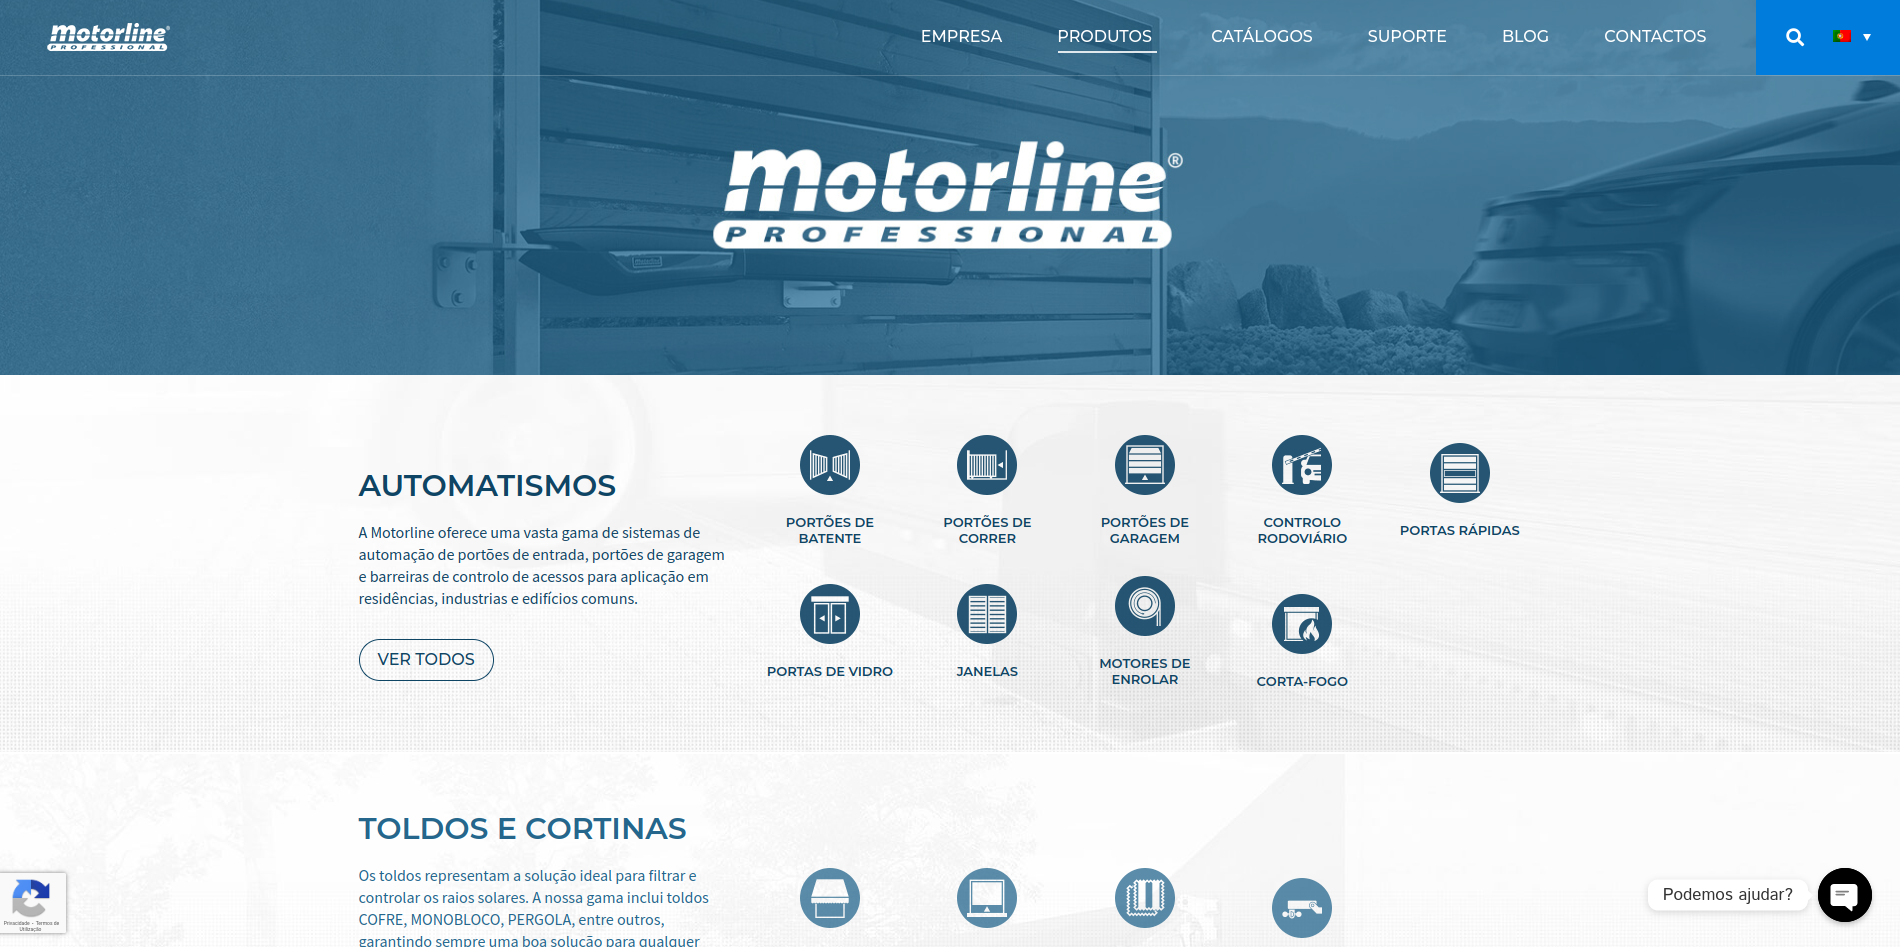
\includegraphics[width=0.55\textwidth]{images/implementacao/scraper/pagina_geral_produtos.png}
    \caption{Página geral de produtos}
    \label{fig:50}
\end{figure}

Sendo assim já é possível identificar cada categoria e subcategoria, assim como também o url da página de produtos
para cada subcategoria. Mas após alguma análise dos dados foi percebido que estas não contem acentuação devido à 
sua formatação no website. Para resolver este problema foi pesquisado por ferramentas capazes de corrigir estes
erros ortográficos. Pelo que foi descoberto que a biblioteca mais utilizada em python para resolver este problema 
é a biblioteca spellchecker, esta ferramenta é a mais utilizada devido à sua capacidade de corrigir erros ortográficos
em diversas linguagens. Sendo assim sempre que uma categoria e subcategoria é obtida, antes de ser guardada, esta é corrigida.

Após isto cada url é aberto e são obtidos os urls de produtos e imagens de amostra dos produtos, para isto foi obtido todos os
elementos clicáveis existentes na secção de produtos de cada página, sendo que cada um correponde a um produto, para obter o nome
do produto correspondente foi utilizado o nome contido no url da página de produto, sendo que todos os produtos seguem a mesma 
estrutura, sendo esta, /produtos/nome-produto. Sendo que em urls não é permitido utilizar acentuação e espaços, então todos os 
nomes foram corrigidos utilizando a mesma ferramenta mencionada anteriormente.

\begin{figure}[htb]
    \centering
    
    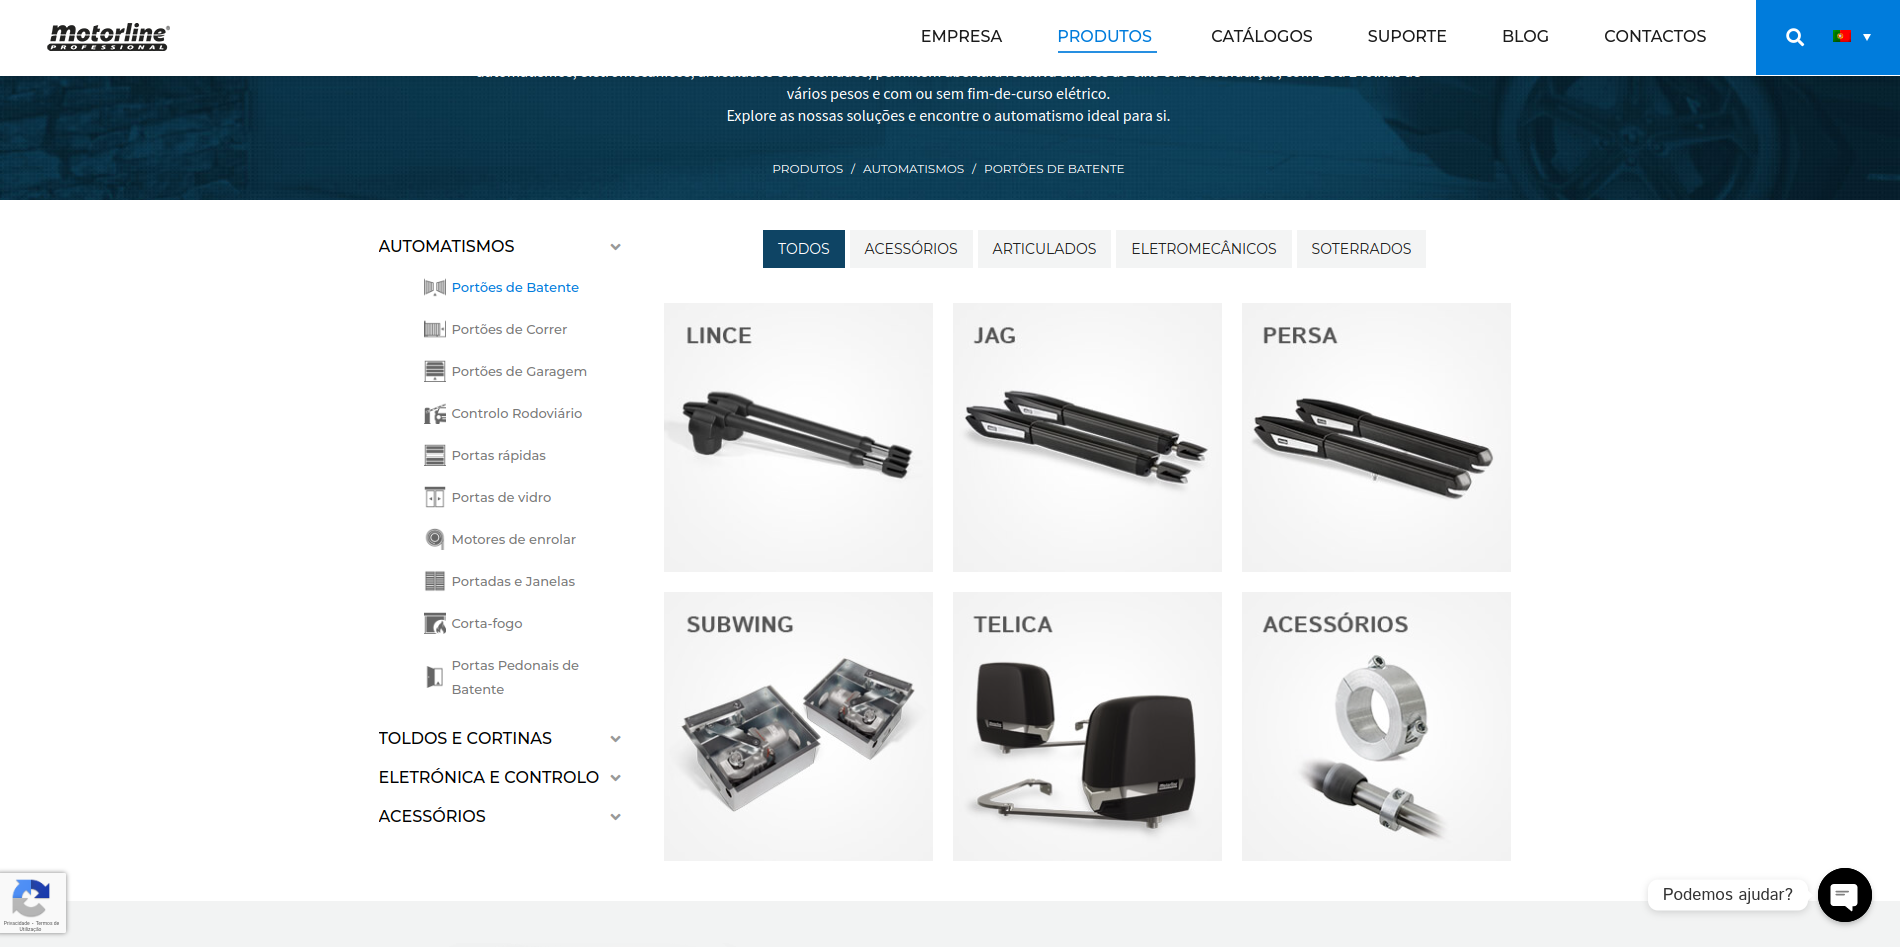
\includegraphics[width=0.55\textwidth]{images/implementacao/scraper/pagina_produtos_subcat.png}
    \caption{Página de produtos de uma subcategoria}
    \label{fig:51}
\end{figure}

\newpage
Neste momento após correr o código foi percebido que existiam algumas páginas de produtos em que este não conseguia obter produtos,
pelo que um erro era atirado, para perceber exatamente que páginas de produtos este erro acontecia, sempre que um erro era detetado
este url seria adicionado a uma nova chave do dicionario mencionado anteriormente, esta chave tem o nome misses e contém todos os urls
em que algum erro aconteceu. Foi então neste momento que foi percebido que nem todas as páginas de produtos são iguais e após uma
reunião com o cliente este expôs que existem páginas de produtos e de detalhes de produtos que são muito diferentes das restantes.

\begin{figure}[htb]
    \centering
    
    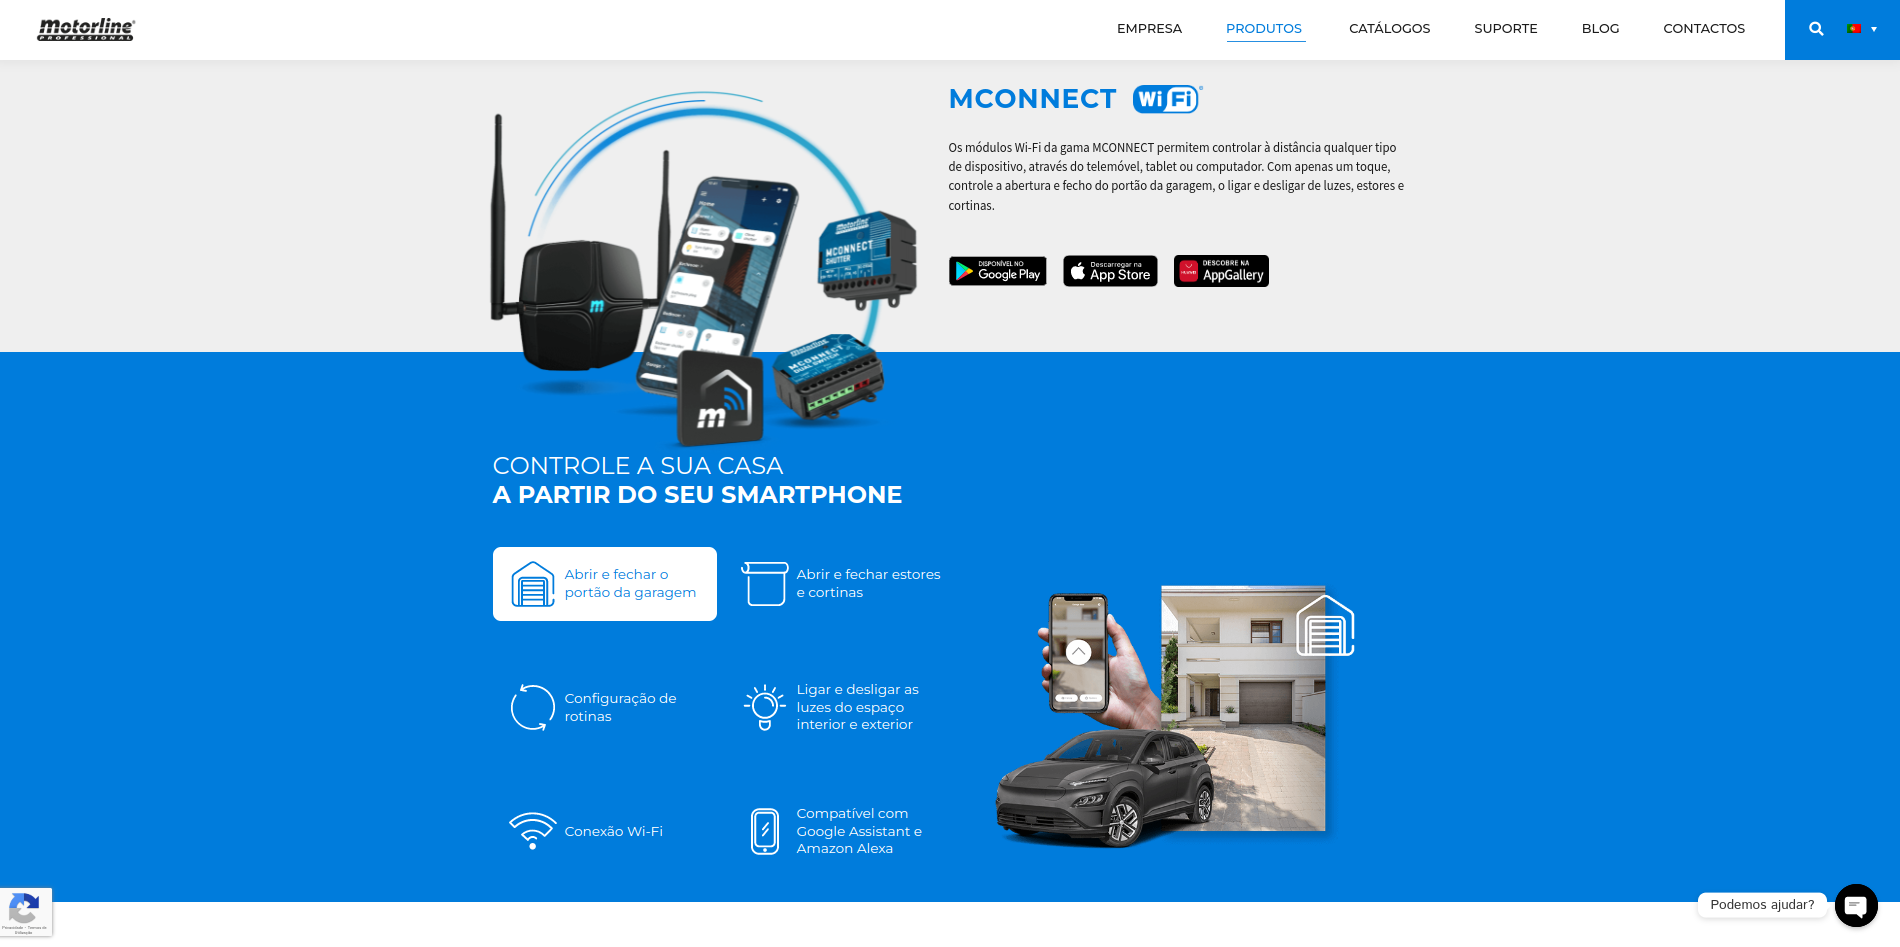
\includegraphics[width=0.7\textwidth]{images/implementacao/scraper/pagina_mconnect.png}
    \caption{Página de produtos de uma subcategoria distinta}
    \label{fig:52}
\end{figure}

De forma ao restante do projeto não ser atrasado foi então decidido primeiramente obter todos os produtos que contêm páginas semelhantes,
sendo assim para cada página de produto foi obtido o titulo que corresponde ao nome do produto, de seguida foi obtida a descrição do produto,
o elemento que contém esta tem como id produto-descrição. As imagens dos produtos são disponibilizadas através de urls na secção da galeria do produto, sendo assim são obtidas todas as imagens desta
galeria e de seguida todos os seus urls.

A documentação dos produtos pode ser disponibilizada através de urls para os manuais,
ou com uma lista dropdown com todos os manuais disponiveis para download, sendo assim são obtidos todos os urls da secção de documentação, 
assim como os seus nomes e todas as opções de documentação do dropdown se este existir.

\begin{figure}[htb]
    \centering
    
    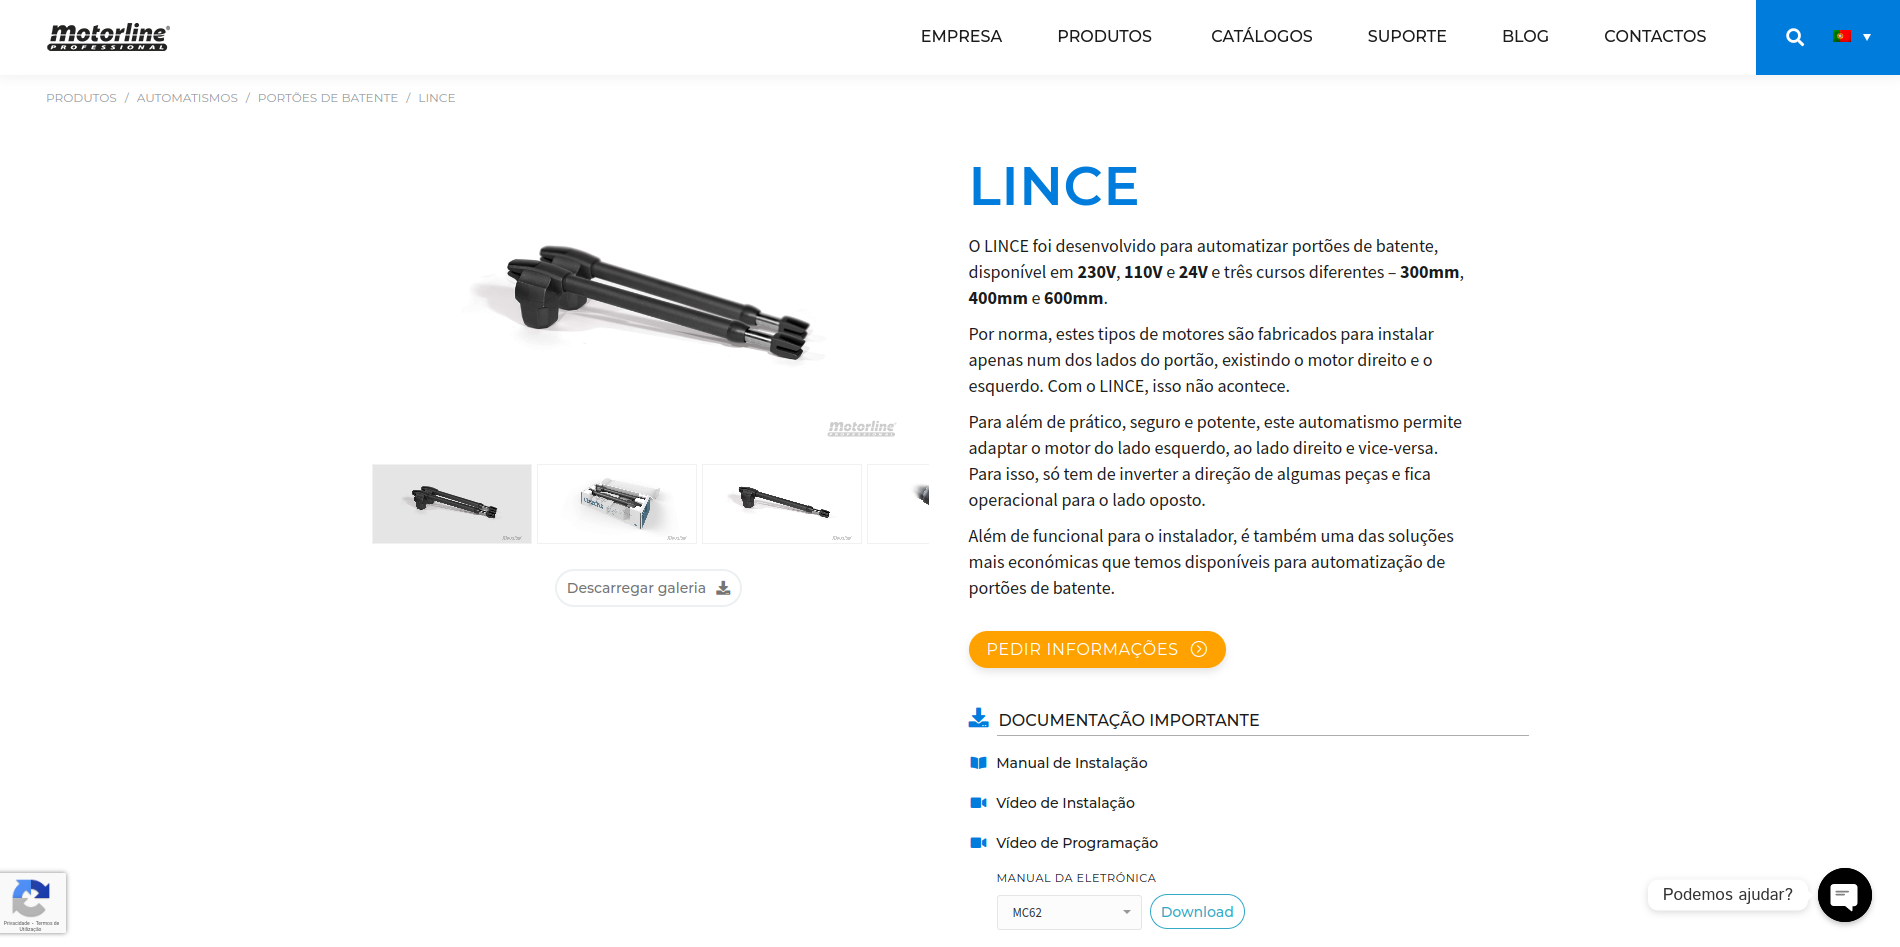
\includegraphics[width=0.7\textwidth]{images/implementacao/scraper/pagina_detalhes_produto.png}
    \caption{Página de detalhes de produto, secção inicial}
    \label{fig:53}
\end{figure}

\newpage

As imagens de desenho técnico e informação geral estão disponibilizadas na secção correspondente
ao nome de cada uma, sendo assim obtidas estas secções e caso estas existam são obtidas as imagens e os seus urls.

\begin{figure}[htb]
    \centering
    
    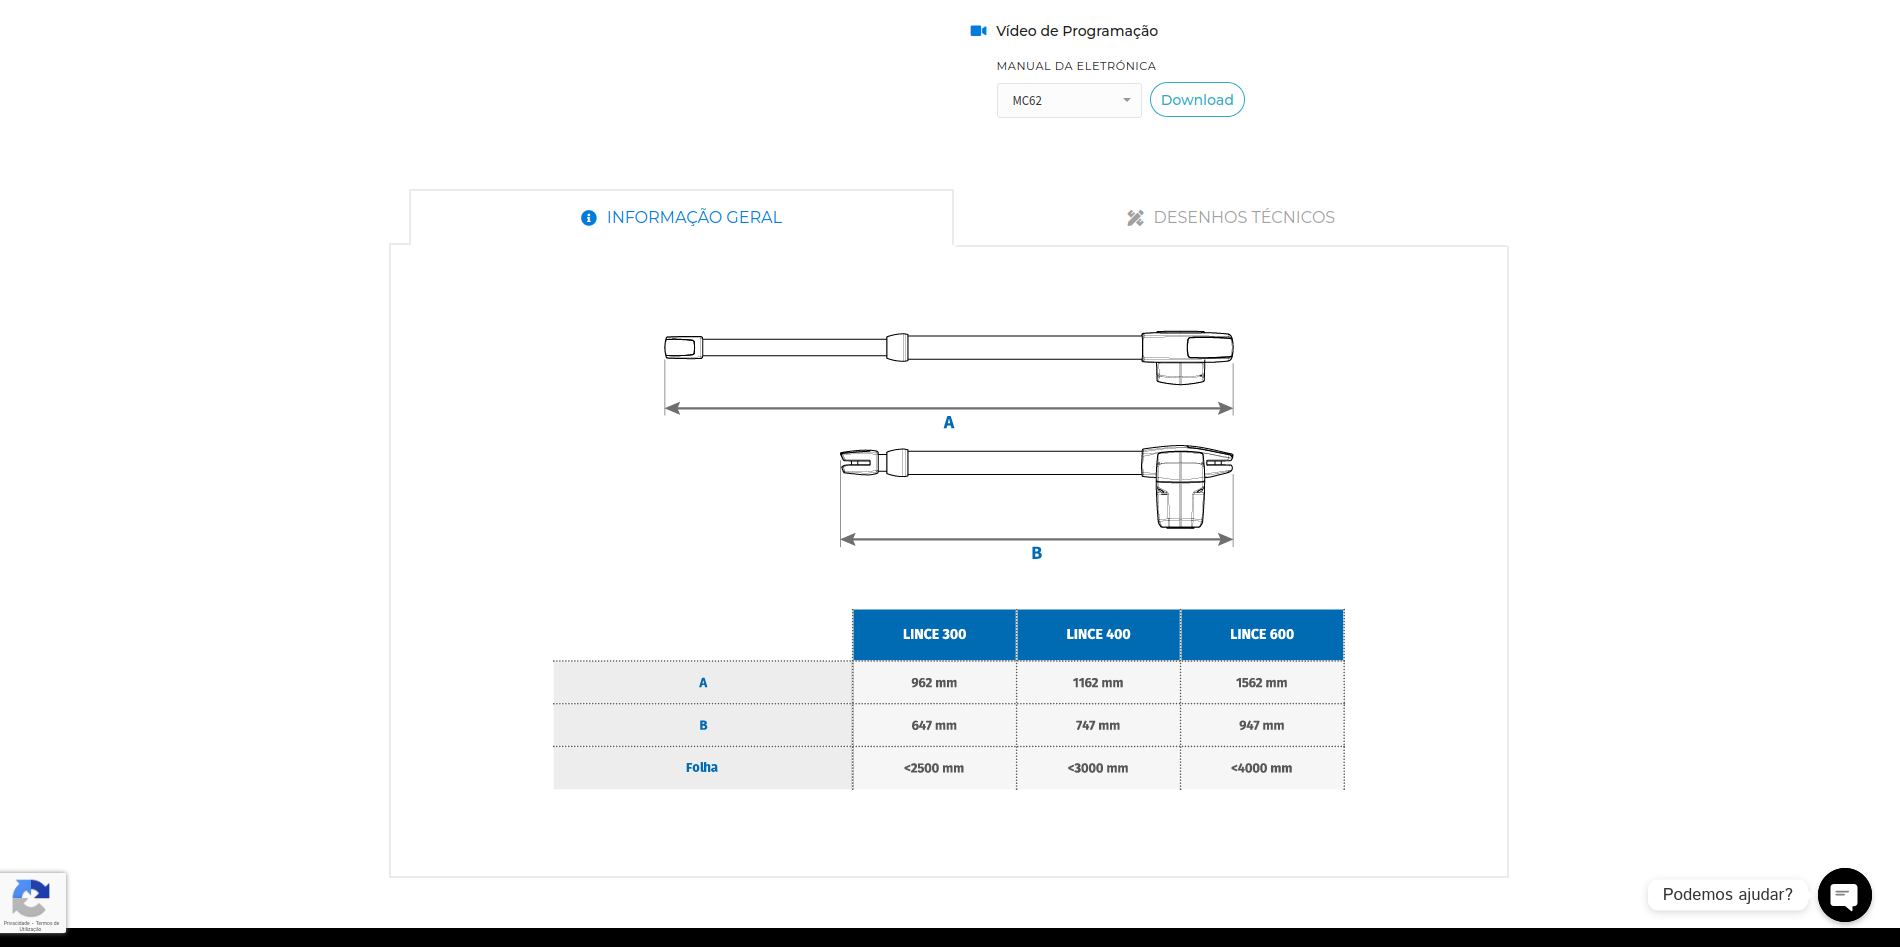
\includegraphics[width=0.7\textwidth]{images/implementacao/scraper/pagina_detalhes_desenhos.png}
    \caption{Página de detalhes de produto, secção de informações}
    \label{fig:54}
\end{figure}

Os videos de produtos estão disponiveis na secção de videos, sendo que cada secção de videos contém o nome do video e por sua vez o video.
Estes videos são demonstrados utilizando um elemento iframe, este elemento contém um url para o video, mas após tentar visualizar este url,
foi percebido que não é possivel obter o vídeo a partir deste. Sendo assim foi investigada a plataforma vimeo, esta é a plataforma que contém
todos os videos de produtos, pelo que para cada um é gerado um id unico e este poderá ser acedido através do url geral da plataforma seguido 
do id do video. Este id está também colocado no elemento iframe, pelo que este é obtido e acrescentado ao url da plataforma conseguindo assim
guardar todos os videos de produtos.

\begin{figure}[htb]
    \centering
    
    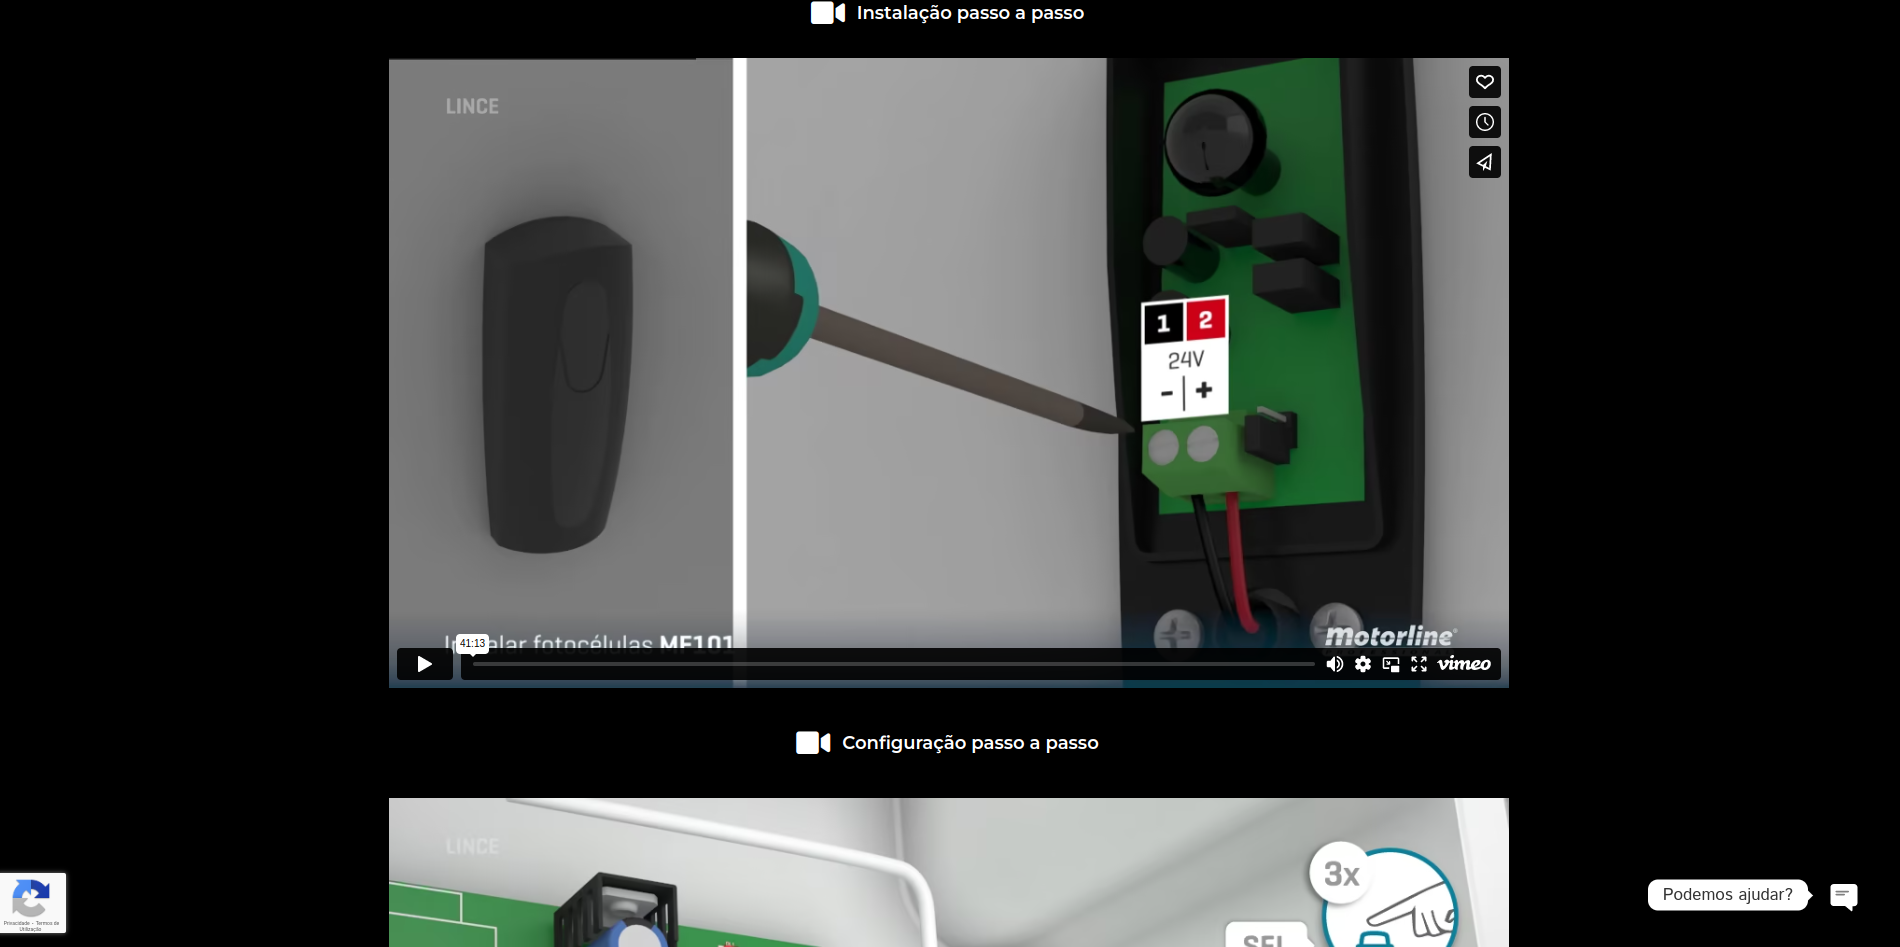
\includegraphics[width=0.7\textwidth]{images/implementacao/scraper/pagina_detalhes_videos.png}
    \caption{Página de detalhes de produto, secção de videos}
    \label{fig:55}
\end{figure}

\newpage

\subsubsection{Implemenção no website}

Após se verificar que eram obtidos pelomenos 80\% dos produtos totais foi então decidido testar no website. Para isto foi utilizada a biblioteca
requests, com a qual é realizado um pedido get a cada url necessário para se obter a página web. Assim que o código foi corrido e a resposta analisada
foi percebido que o website bloqueia este tipo de solução recebendo a resposta demonstrada pela figura~\ref{fig:56}

\begin{figure}[htb]
    \centering
    
    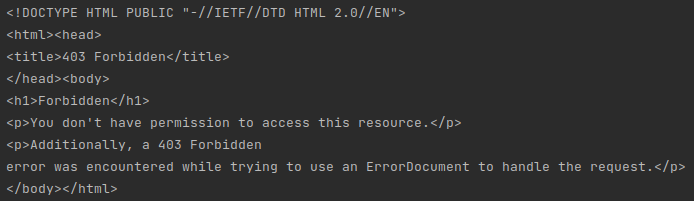
\includegraphics[width=0.7\textwidth]{images/implementacao/scraper/forbiden_response.png}
    \caption{Resposta obtida aquando o pedido ao url da página web}
    \label{fig:56}
\end{figure}

Através da resposta obtida foi então percebido que seria necessário alterar a abordagem visto que a abordagem anterior não seria possível utilizar.
A abordagem opcional a seguir seria simular a ação humana abrindo um navegador e pesquisando pelo url desejado. 

Após uma investigação foi descoberto que existem ferramentas que permitem controlar o dispositivo onde correm impedindo a utilização deste enquanto se 
encontram a correr, assim como ferramentas que apenas recebem o navegador a utilizar e abrem uma nova janela deste navegador para realizar a pesquisa.
Visto que o processo de obter os produtos seria demorado, foi optado pela segunda opção visto que seria possivel continuar com trabalho em paralelo com a
obtenção de dados. Sendo assim a ferramenta mais recomendada para realizar esta operação é a biblioteca selenium, esta biblioteca permite realizar exatamente
o processo referido anteriormente com a possibilidade de escalar com multi threading, permitindo abrir diversas janelas do navegador simultaneamente,
diminuindo drasticamente o tempo de execução para obter os dados, esta funcionalidade não foi explorada devido a limitações de hardware, 
mas seria uma importante implementação futura.

Utilizando a biblioteca selenium foi primeiramente indicado qual o navegador a utilizar, neste caso foi escolhido o chrome devido a este já estar instalado
no dispositivo. Após se indicar qual o navegador a utilizar, é necessário para cada página indicar qual elemento esperar que carregue, pois assim que a pesquisa
é efetuada a página poderá demorar a carregar pelo quem se deverá indicar a espera pelo elemento que se deseja obter. Visto que a página carregada poderá não
conter o elemento a obter foi então implementado um tempo de espera máximo de 5 segundos, assim que este tempo expira a operação é abortada e o url é adicionado
à lista de urls com erros.

\newpage

\subsubsection{Armazenamento de dados}

Após se obter os dados dos produtos, é necessário guardar estes na base de dados para disponibilizar para a sua utilização no backend. Para realizar
esta operação existem duas opções, criar um serviço para inserir produtos e realizar um pedido a este serviço, ou então conectar diretamente
o web scraper à base de dados. Visto que não seria de grande interesse conectar diretamente à base de dados, foi decidido criar um serviço que recebe um produto e o 
insere na base de dados. O grande problema que surgiu com esta solução é que os pedidos ocorrem de forma sequencial, mas com pouco tempo de espera entre estes, o que
levava a que o limite máximo de conexões com a base de dados fosse extrapolado. Isto acontece porque para cada serviço chamado é criado uma nova conexão à base de 
dados, todas as operações são realizadas e por fim a conexão é terminada, mas enquanto estas operações estão a decorrer, o servidor poderá receber mais pedidos, o que 
leva a que mais conexões sejam criadas, atingindo assim rápidamente o limite de conexões da base de dados. Como solução para este problema surgiu a ideia de receber todos
os produtos a inserir em apenas um pedido e inserir estes na base de dados.

\subsubsection{Melhoria de implementação}

Após se completar o processo foi então decidido melhorar a implementação resolvendo os erros encontrados em urls especificos. De forma a perceber exatamente quais os urls
que possuem erros foi então direcionado os dados obtidos para um ficheiro json. Sendo assim os urls com erros eram os indicados na figura~\ref{fig:57}.

\begin{figure}[htb]
    \centering
    
    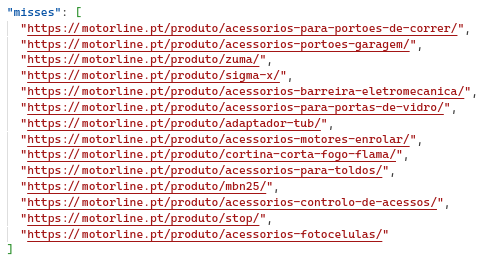
\includegraphics[width=0.7\textwidth]{images/implementacao/scraper/urls_erro_iteracao_1.png}
    \caption{Urls com erro primeira interação}
    \label{fig:57}
\end{figure}

Após uma primeira análise foi possível perceber que grande maioria dos erros provém de urls de acessórios de produtos, isto deve-se ao facto de os acessórios de produtos encontrarem-se
na página de produtos de subcategoria e serem tratados como um url de detalhes de produto, sendo assim sempre que se trata de um url de acessórios seria necessário correr código para 
obter dados de destes ao invés de detalhes de produtos. Para desenvolver este código foi primeiramente analisada a página de acessórios de produtos(Figura~\ref*{fig:58}), 
esta página contém para cada acessório um elemento do tipo artigo o qual contém uma imagem, titulo e descrição, esta descrição por vezes contém urls para os produtos aos quais este acessório se refere, pelo que sempre que estes
urls são detetados, os nomes dos produtos são guardados para futuramente realizar a ligação entre os acessórios e os produtos, visto que não existem produtos com nomes iguais. Foi percebido que nos urls a palavra accessórios está 
sempre contida pelo que sempre que esta é detetada em um url é corrido o código referente à obtenção de acessórios.

\begin{figure}[htb]
    \centering
    
    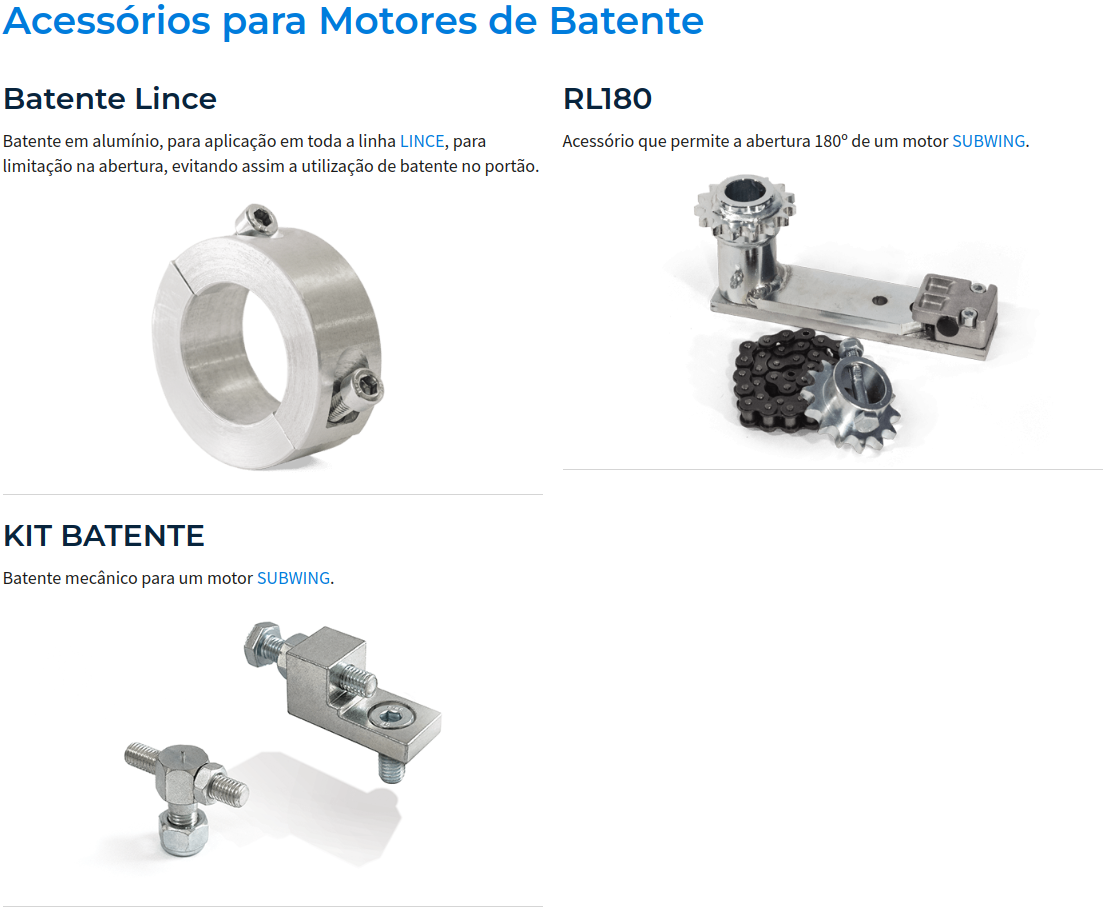
\includegraphics[width=0.55\textwidth]{images/implementacao/scraper/pagina_acessorios.png}
    \caption{Exemplo de página de acessórios}
    \label{fig:58}
\end{figure}

%\newpage

Após correr o novo código criado foi percebido que a quantidade de urls com erros diminuiu, mas existiam produtos com páginas de detalhes de produtos comuns pelo que estas foram analisadas e foi percebido
que um erro ocorria devido a por vezes as páginas não conterem vídeos ou imagens de documentação, sendo que o código foi alterado para apenas obter estes dados se os elementos existirem na página. 
Após correr novamente o código foi percebido que a quantidade de falhas obtidas diminuiu drásticamente (Figura~\ref{fig:59}). Mas mesmo assim ainda existiam 3 falhas a ocorrer e após uma análise foi percebido que
estas falhas estavam a ocorrer devido a:

\begin{enumerate}
    \item Uma página de subcategoria de produtos conter um serviço;
    \item Um produto conter uma página de detalhes de produto com sub produtos;
    \item Existir uma página de adaptadores de produtos;
    \item Um produto conter uma página de detalhes diferente das demais;
\end{enumerate}

\begin{figure}[htb]
    \centering
    
    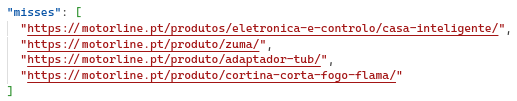
\includegraphics[width=0.65\textwidth]{images/implementacao/scraper/melhor_corrida.png}
    \caption{Exemplo de página de acessórios}
    \label{fig:59}
\end{figure}

\newpage

Visto que a página de adaptadores de produtos segue uma estrutura similar à estrutura dos acessários este foi o primeiro a ser abordado e resolvido, correndo o código de obter detalhes de acessórios sempre a 
palavra acessórios ou adaptadores se encontra no url. De seguida foi percebido que para resolver o problema de existerem serviços e subprodutos o diagrama de base de entidade relação teria de ser alterado pelo que
primeiramente foi resolvido o problema do produto que contém uma página de detalhes diferente das demais. 

Este produto para além da dificuldade de ser uma página completamente diferente as informações encontram-se espalhadas pela página (Figura~\ref*{fig:60}), pelo que estas deveriam ser combinadas para construir os detalhes do produto.

\begin{figure}[htb]
    \centering
    
    
\includegraphics[width=0.7\textwidth]{images/implementacao/scraper/flama.png}
    \caption{Exemplo de página de produto incomum}
    \label{fig:60}
\end{figure}

\newpage

\section{Serviços Backend}

De forma a realizar a integração entre a aplicação \emph{frontend} e os dados, foi necessário desenvolver
uma API para dar suporte a todos os serviços necessários para a aplicação.
API sigla para \emph{Application Programming Interface} disponibiliza um conjunto de funções e
dados que facilita as interações entre aplicações e permite que troquem informação ~\cite{rest_cookbook}.
Esta ferramenta apesar de ser desenvolvida para trabalhar em conjunto com outros programas, ela são
em sua grande maioria desenvolvidas para serem entendidas e utilizadas por outros programadores no
desenvolvimento dos seus programas ~\cite{api_design}.

\subsection{Serviços REST Full}
Explicar o que é

\subsection{Organização do projeto}
Antes de iniciar a implementação, foi definido qual a estrutura de projeto a seguir, pelo que a esoclhida
foi MVC devido a ser a mais comum e estabelecida. Sendo assim a organização do projeto segue a seguinte estrutura:
\begin{figure}[htb]
  \centering
  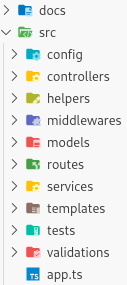
\includegraphics[width=0.2\textwidth]{images/implementacao/api/project_organization.png}
  \caption{Exemplo de página de produto incomum}
  \label{fig:61}
\end{figure}

\begin{itemize}
  \item \textbf{docs} - Documentação gerada;
  \item \textbf{src} - Base de todo o projeto;
  \item \textbf{config} - Ficheiros de configuração do projeto;
  \item \textbf{controllers} - Controladores para cada pedido;
  \item \textbf{helpers} - Ficheiros com funções gerais utilizadas regularmente;
  \item \textbf{middlewares} - Ficheiros com os middlewares da api;
  \item \textbf{models} - Classes criadas para representação de base de dados e para as entidades de resposta;
  \item \textbf{routes} - Rotas existentes;
  \item \textbf{services} - Serviços para cada pedido;
  \item \textbf{templates} - Templates de email a serem enviados;
  \item \textbf{tests} - Testes de código realizados;
  \item \textbf{validations} - Validações a realizar a nível de modelo de negócio e validação de dados;
  \item \textbf{app} - Ficheiro de início do projeto;
\end{itemize}

\subsection{Definição de rotas base}
Após a definição da estrutura do projeto foi então definido as rotas base a existir, estas são rotas
que se referem a cada tipo de utilizador. Para melhor organização destas rotas e aplicação de regras foram definidos 3 routers,
user para utilizadores se sessão, professional para técnicos e company para empresas. De forma a definir para o projeto qual o router a utilizar
em cada pedido foi então definido que:
\begin{itemize}
  \item \textbf{http://baseurl:port/professional} - Encaminhar para router de técnicos;
  \item \textbf{http://baseurl:port/company} - Encaminhar para router de empresas;
  \item \textbf{Restantes} - Encaminhar para router de user;
\end{itemize}

\subsection{Middlewares} 
Um middleware comporta-se como uma ligação entre porções de código, sendo possível este também executar código.

\subsubsection{Linguagem}
O bem mais essencial em uma boa comunicação entre duas partes é a utilização da mesma linguagem, sendo assim foi necessário perceber
qual a linguagem a utilizar quando se responde a um pedido. Para este fim foi então desenvolvido um middleware,
o objetivo deste é verificar se existe a chave language no cabeçalho do pedido, caso esta exista é então obtido a linguagem e guargada
nas variáveis locais do pedido. Em caso de esta tag não existir, foi então decido que a aplicação responderá em português por omissão,
este valor poderá ser futuramente alterado de forma simples.

\subsubsection{Autenticação}
De forma a assegurar a autenticação dos utilizadores que necessitam desta foi então decidido implementar JsonWebToken,
este tipo de autenticação baseia-se em a utilização de tokens com tempo de expiração, sendo que enquando o token estiver válido,
o utilizador poderá realizar pedidos e assim que este token expirar este terá de se autenticar novamente para obter um novo token.
A utilização de tokens permite também assegurar que os pedidos são realizados com tokens gerados pela api através de utilização de uma chave
de assinatura de token, impedindo assim a utilização de tokens gerados por utilizadores.
\begin{figure}[htb]
  \centering
  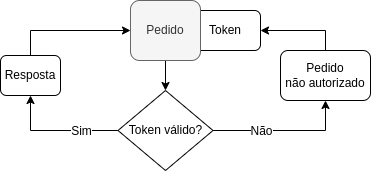
\includegraphics[width=0.5\textwidth]{images/implementacao/api/jwt_session.png}
  \caption{Exemplo de página de produto incomum}
  \label{fig:62}
\end{figure}

A grande valia da utilização a técnica de autenticação mencionada anteriormente é a segurança desta, mas este nivel de segurança
leva a que as aplicações que não necessitam de um nivel de segurança muito alto se tornem impráticas. Isto acontece porque estes 
tokens têm geralmente uma duração muito curta como por exemplo 15 minutos, e sempre que um token de sessão expira o utilizador 
teria de realizar novamente o login.

A solução deste problema sem a perda de segurança significativa veio pelo meio da utilização de tokens de duração maior em conjunto 
com os tokens de duração curta, sendo que enquanto o token de grande duração estiver válido, novos tokens de curta duração são gerados 
para o utilizador nunca perdendo assim a sua sessão. Estes tokens de grande duração tem por nome tokens de refresh e os tokens de curta 
duração têm por nome tokens de sessão. Sempre que o utilizador termina a sua sessão o token de refresh deverá ser apagado.

Sempre que um utilizador realiza um pedido o seu token de sessão deverá ser validado, caso este seja válido, o seu token de refresh deverá 
também ser validado e apenas após isto o utilizador estará autenticado. Caso o token de sessão ou de refresh esteja expirado, este continuará
a estar sem autorização para realizar o pedido, mas poderá pedir um novo token de sessão enquanto o seu token de refresh estiver válido, 
isto acontece sem realizar novamente o login e sem o utilizador perceber.